\section{Fans are Unavoidable}

\pat{I propose to kill this section, unless there is a short proof that a pathwidth-$2$-partition of some planar graph (probably the LMST graph) must contain a large fan-minor.} \david{I am leaning towards killing it too, I have adminstered the last rites by moving it to an appendix, but will try one more attempt at a proof before giving the final blow. }

\david{I suspect the lower bound can be pushed further to show  that fan graphs really are best possible. Conjecture: there exist $n$-vertex planar graphs such that for any graph $H$, if $G$ is contained in  a $\tilde{O}(\sqrt{n})$-blowup of $H$, then $H$ contains a fan on $\Omega(n^c)$ vertices, for some $c>0$, possibly $c=\frac12$. Here I try to prove this where $G$ is from \citep{LMST08}. }

\begin{lem}[\citep{LMST08}]
\label{FindPath}
Let $G$ be a near-triangulation. Let $S\subseteq V(G)$ such that $G[S]$ is connected. If two vertices $u,v\in N_G(S)$ are in the same component of $G-S$, then there is a $uv$-path in $G[ N_G(S) ]$.
\end{lem}

\citet{LMST08} defined the following planar graph. Fix $k\in\mathbb{N}$. Start with a $k^2 \times k$ triangulated grid $Z$. Let $C_1,\dots,C_{k^2}$ be the columns of $Z$, and let $R_1,\dots,R_k$ be the rows of $Z$. So $|C_i|=k$ and $|R_i|=k^2$. Let $v_i$ be the vertex in $C_i$ in the top row of $Z$. Add a disjoint path $P$ on $k^3+1$ vertices and $k^3$ edges. Break $P$ into $k^2$ edge-disjoint subpaths $P_1,\dots,P_{k^2}$, each with $k$ edges. Add an edge between $v_i$ and each vertex in $P_i$.
Each set $C_i\cup P_i$ is called a \defin{rib}. Finally, add one vertex $r$ adjacent to every vertex in $P$. The resulting graph $G$ is a planar near-triangulation on $2k^3+1$ vertices.

\pat{For this graph, $n:=2k^3+1$, and this graph has an $H$-partition $\{V_x:x\in V(H)\}$ of width $w\in O(\sqrt{n})$ such that $H$ has bounded pathwidth (even treedepth) and the longest path in $H$ has length $O(1)$.  Here it is:\\[2ex]
Let $V_a:=\{r\}$.  Let $V_0$ be the vertex set of $\sqrt{k}+1$ equally spaced ribs that includes the first rib and the last rib. Then $|V_0|=2k(\sqrt{k}+1)=O(k^{3/2})$ and $G_1:=G-(V_a\cup V_0)$ has $\sqrt{k}$ components $C_1,\ldots,C_{\sqrt{k}}$, each of which contains $O(k^2/\sqrt{k})=O(k^{3/2})$ ribs.  For each component $C_i$, we again choose $\sqrt{k}+1$ equally spaced ribs, including the first and last rib, and put these in a bag $V_{1,i}$.  Then the components of $G_2:=G_1-(\bigcup_{i=1}^{\sqrt{k}} V_{1,i})$ each contain $O(k^2/k)=O(k)$ ribs.  At this point the graph $H$ is an apex star where $a$ is the apex vertex, $V_0$ is the root, and $V_{1,1},\ldots,V_{1,\sqrt{k}}$ are leaves.  Repeating this once more on each component of $G_2$ gives sets $V_{2,1},\ldots,V_{2,k}$. The graph $G_3:=G_2-(\bigcup_{i=1}^{k} V_{2,i})$ has components that each contain $O(\sqrt{k})$ ribs. Now the graph $H$ is an apex tree of height $2$.  Finally, put each component of $G_3$ in its own part.  Now $H$ is a $1$-subdivision of an apex tree of height $2$, where only the edges adjacent to the leaves are subdivided.  Any path in $H$ consists of at most two paths in $H-a$ (a tree of height $3$) joined at $a$.  So every path in $H$ has length at most $2\times 6 + 2 = 14$.  (Being a little more careful gives an upper bound of $12$, I think.)}

\david{Nice. If you include the apex vertex in $V_0$, then the quotient has treedepth 4 and pathwidth 3. \\
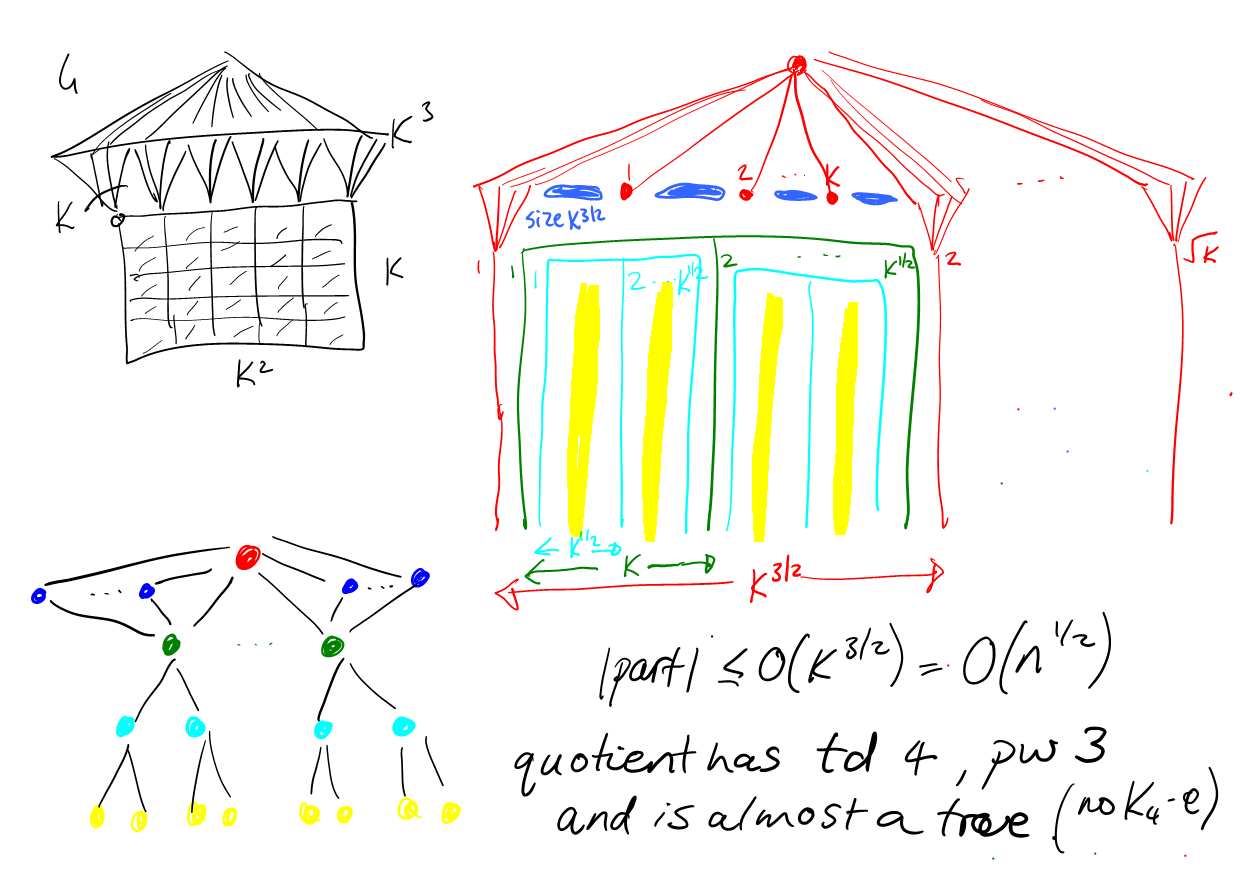
\includegraphics[page=1,width=\textwidth]{sqrtnTreePartitions.pdf}
}

\pat{Two directions:
\begin{compactenum}
    \item Try to show that for any $H$-partition of width $\tilde{O}(\sqrt{n})$ where $\pw(H)\le 2$, $H$ contains an $n^{\epsilon}$ fan minor. \david{surely this is true}\\[2ex]
    % \pat{I'm attempting to prove this below.}
    %
    %
    % Your argument, in the paragraph below, can be completed to finish this.  Look at the large set of ribs that are avoided by $V_a$ and in one component $C$ of $G-V_a$.  Let $C'$ be a tree that is contained in $C$ and that contains all the vertices of the ribs in $C$.  Let $H[C']$ be the subgraph of $H$ induced by the bags that intersect $C'$.
    % Every rib, except the first and the last rib separates $C'$ into at least two non-empty parts.  Suppose $V_x$ is a bag that contains a top vertex (a vertex of $P$) of one of these ribs but $V_x$ does not contain the entire first rib or the entire last rib. Then $x$ has degree at least $2$ in $H[C']$.  Doing contractions doesn't increase pathwidth, so we can contract any edge of $H[C']$ incident to a vertex $x$ whose bag does not contain a top vertex.  Now we have a graph $H'\subseteq H[C']$ and $H'+a$ is a minor of $H$.
    % I claim that $H'$ has at most $2$ nodes of degree less than $2$. Continue... \\[2ex]
    % The contractions done to create $H'$ never reduce the number of bags that contain a top vertex.  We started with $\Omega(k^4/w^2)$ of these bags and they're all still there.  This means that $H$ contains a minor $H'+a$ that consists of a connected graph with one dominating vertex $a$, $H'$ has pathwidth $1$, and at most two vertices of $H'$ have degree less than $2$.  So $H'$ is a caterpillar with at most $2$ leaves.  Therefore $H'$ is a path on $\Omega(k^4/w^2)=\tilde\Omega(n^{1/3})$ vertices, for any $w\in \tilde{O}(\sqrt{n})$.\\[2ex]
   \david{note that the $n^{2/3}\times n^{1/3}$ grid with a vertex dominating the top row has a $T$-partition of width $O(n^{1/2})$, where $T$ is a tree with treedepth 4 and pathwidth 3.\\
   \includegraphics[page=2,width=\textwidth]{sqrtnTreePartitions.pdf}
   } \\[2ex]
   \pat{It's even worse than that.  It has an $H$-partition where $H$ is a subdivided star (so $H$ has pathwidth $2$).  To see this, make one bag $V_a$ that contains the apex vertex $a$ and contains $n^{1/6}$ equally-spaced columns so that $G-V_a$ is a set of $n^{1/2}\times n^{1/3}$ grids.  Now make a path-partition of each of these grids by repeatedly peeling away the outer layer.  Then only the first part of each path partition is adjacent to vertices in $V_a$.}
  \item Try to find a $H$-partition of width $O(\sqrt{n})$ (no logs) where $\pw(H)$ is bounded.
  \end{compactenum}
}




% \pat{Actually, the hierarchy of separators used in the $H$-partition described above shows that any interesting example has to have treewidth $\tilde{\Omega}(\sqrt{n})$.  If $G$ has treewidth $n^{1/2-\epsilon}$ then you get an $H$-partition of $G$ of width $O(\sqrt{n})$ where $\td(H)\in O(1/\epsilon)$ using hierarchical separators.  I guess this is what David and Zdenek do \david{correct}.  \\[2ex]
% Maybe this is how we should have approached the problem from the start.  Take the separator $S$ of size $c\sqrt{n}$ that minimizes the size of the largest component in $G-S$.  Repeat this on each component of $G-S$ whose size is greater than $n^{1-\epsilon}$ (or, if you prefer, the components whose treewidth is greater than $n^{1/2-\epsilon}$).  This gives a separator tree $T$.  Look at the height $h$ of the largest complete binary tree minor contained in $T$.  Then $\pw(H)=h+O(1/\epsilon)$.  Argue that, if $h\in\omega(1)$ then $G$ is basically a grid, so it has bandwidth $O(\sqrt{n})$.  (Note that $h=O(\log\log n)$ if $G$ is the $\sqrt{n}\times\sqrt{n}$ grid.)} \david{the ``is basically a grid'' step looks challenging} \pat{I think the correct word is ``hopeless.''}



Consider an $H$-partition $(V_x:x\in V(H))$ of $G$ with width $w$. Let $V_a$ be the part containing $r$. Let $S$ be the connected component of $G[V_a]$ containing $r$. Since $|S|\leq |V_a|\leq w$, at most $w$ ribs intersect $S$, and thus at least $k^2-w$ ribs avoid $S$. That is, there exists $I\subseteq \{1,\dots,k^2\}$ such that $|I|\geq k^2-w$, and $C_i\cup P_i$ avoids $S$ for every $i\in I$. Since $|S|\leq w$ and there are $k$ rows, some row $R_i$ has at most $w/k$ vertices in $S$. It follows \david{prove this} that the $S$-free ribs are contained in at most $(w/k)+1 \leq 2w/k$ components of $G-S$. Hence, there is a set $J\subseteq I$ such that $|J|\geq k(k^2-w)/2w$ and all the ribs $\{P_i\cup C_i:i\in J\}$ avoid $S$ and are in the same component of $G-S$. Let $X:=\bigcup\{V(P_i):i\in J\}$. So $|X|\geq k|J|\geq k^2(k^2-w)/2w$. Every vertex in $X$ is adjacent to $r$, and thus $X\subseteq N_G(S)$. Thus $X$ is a set of at least $k^2(k^2-w)/2w$ vertices in $N_G(S)$ and in the same component of $G-S$. By \cref{FindPath}, there is a connected subgraph $Y$ of $G[N_G(S)]$ containing $X$. Let $R:=\{ b\in V(H): V_b\cap V(Y)\neq\emptyset\}$. So $|R|\geq |V(Y)|/w\geq |X|/w \geq k^2(k^2-w)/2w^2$. Since $V(Y)\subseteq N_G(S)$, we have $R\subseteq N_H(a)$. Since $Y$ is connected, $H[R]$ is connected. That is, the vertex $a$ has at least $k^2(k^2-w)/2w^2$ neighbours in $H$ that induce a connected subgraph of $H$.
\david{note that if $w\leq O(k^{3/2})$ (which we may assume), then $|R|\geq (\frac12 -o(1))k$ which is $\Omega(n^{1/3})$, but $R+a$ is not quite a fan in $H$, we want $R$ to be a long path, what if $R$ is a star? }



\david{try again...}
Consider an $H$-partition $(V_x:x\in V(H))$ of $G$ with width $w$. Let $V_a$ be the part containing $r$. Let $S$ be the connected component of $G[V_a]$ containing $r$.
Consider a component $X$ of $S-r$. Let $X^+$ be the subgraph $G[V(X)\cup\{r\}]$. Suppose there exists a component $C$ of $G-S$ such that for every edge $vw$ of $G$, if $v\in V(X)$ and $w$ is in the outerface of $X^+$, then $w$ is in $C$. Then we say that $X$ is \defin{surrounded} (by $C$). A rib $P_i\cup C_i$ is \defin{$S$-free} if $V(S)\cap (P_i\cup C_i)=\emptyset$.

Every $S$-free rib is contained in some component of $G-S$.
For each component $C$ of $G-S$, define the \defin{weight} of $C$ to be the number of $S$-free ribs in $C$ minus the number of components of $S-r$ surrounded by $C$. Since $|S|\leq |V_a|\leq w$, at most $w$ ribs intersect $S$, and thus at least $k^2-w$ ribs are $S$-free. Every surrounded component of $S-r$ has a vertex in $P\cap V(S)$. So there are at most $|V(S)|\leq w$ surrounded components of $S-r$. Hence, the total weight of components of $G-S$ is at least $(k^2-w)-w=k^2-2w$. Since $|S|\leq w$ and there are $k$ rows, some row $R_j$ has at most $w/k$ vertices in $S$. So $R_j-S$ has at most $(w/k)+1\leq 2w/k$ components.

Let $C$ be a component of $G-S$ with positive weight. So at least one $S$-free rib $C_i\cup P_i$ is contained in $C$. Thus, there is a vertex $x$ in $C\cap R_j$. Hence, the component of $R_j-S$ that contains $x$ is contained in $C$. Since there are at most $2w/k$ components of $R_j-S$, there are at most $2w/k$ components of $G-S$ with positive weight. Thus, some component $C$ of $G-S$ has weight at least $k(k^2-2w)/2w$.

Let $I$ be the set of integers $i\in\{1,\dots,k^2\}$ such that the rib $C_i\cup R_i$ is contained in $C$. Let $X_1,\dots,X_t$ be the set of components of $S-r$ surrounded by $C$. So $|I|-t\geq k(k^2-2w)/2w$. Let $Q:=\bigcup\{V(P_i):i\in I\}$. So $|Q|\geq k|I|$. Every vertex in $Q$ is adjacent to $r$, and thus $Q\subseteq N_G(S)$. Note that each component $X$ of $S-r$ surrounded by $C$ breaks the path $Q$. In this case, by \cref{FindPath}, there is a path in $C$ around the underside of $X$ joining up $X$ again \david{too vague}. This loses less than $2k$ vertices from $Q$. We obtain a path $Q'$ in $C$ with $|Q'|\geq |Q|-kt \geq k|I|-kt \geq k^2(k^2-2w)/2w$, where $Q'\subseteq N_G(S)$.
Let $R:=\{ b\in V(H): V_b\cap V(Y)\neq\emptyset\}$. So $|R|\geq |V(Q')|/w\geq k^2(k^2-2w)/2w^2$. Since $V(Q')\subseteq N_G(S)$, we have $R\subseteq N_H(a)$. Since $Q'$ is connected, $H[R]$ is connected. That is, the vertex $a$ has at least $k^2(k^2-2w)/2w^2$ neighbours in $H$ that induce a connected subgraph of $H$. \david{I want to argue that $R$ contains a long path because $Q'$ is a path. }

% \pat{What seems to be missing from both of these arguments is some restriction on $H$. Consider the $1$-stack matching on $V(P)$ whose largest rainbow is of size $O(\log k)$. For each edge of the matching, in decreasing order of length, make the $H$-partition have a bag of size at most $2+2k$ that contains the endpoints $v$ and $w$ of this edge and the at most two columns whose ribs contain $v$ and $w$ (if those columns are not already in some bag). Put $r$ in a bag $V_a$ by itself.  The bags of $H$ corresponding to the matching create a balanced binary tree in $H$ plus edges between siblings (a triangle tree). The longest path in this part of $H$ has length $O(\log k)$.  So the longest fan in $H$ that has $V_a$ as an apex vertex has length $O(\log k)$.  Of course, this isn't an issue for us because this particular $H$ has pathwidth $\Omega(\log k)$, which we don't allow.}




